\documentclass[twocolumn]{article}
\usepackage[utf8]{inputenc}
\usepackage{hyperref}
\usepackage[version=4]{mhchem}
\usepackage{placeins}
\usepackage{graphicx}

\title{Chemistry 2 TP2}
\author{Louis-Hendrik Barboutie}
\date{March 2022}

\begin{document}

\maketitle

\clearpage

\onecolumn

\tableofcontents

\clearpage

\twocolumn

\section{Abstract}
The aim of this experiment is to determine the unknown concentration of a Mohr's salt solution, by the method of colorimetry, by establishing a calibration curve. The concentration has been found to be $(8.460 \pm 0.215) \cdot 10^{-5} \ mol \cdot L^{-1}$. 
\section{Introduction}
The experiment will exploit the property of d-block complexes to be colored. In particular, the complex studied is ferroin (\ce{Fe(o-phenantroline)3SO4}). The method of colorimetry can be applied, where the intensity of light absorbed by a solution can be measured. The absorption of light rises with the intensity of the coloration, which is in turn due to the concentration. This allows us to construct a calibration curve, with which we can identify unknown concentrations bearing the same complexes. \\ The Beer-Lambert law describes this phenomenon: it states that the absorbance depends on the concentration of the solution, the path length of the light going through the solution and on a complex specific constant, the molar attenuation coefficient. 
\section{Experiment}
\subsection{Chemicals}
\subsubsection{Water}
\begin{itemize}
    \item Chemical formula: \ce{H2O}
\end{itemize}
\subsubsection{Ammonium iron(II) sulfate (hexahydrate)}
\begin{itemize}
    \item Also known as Mohr's salt
    \item Chemical formula: \ce{FeSO4,(NH4)2SO4, 6H2O}
    \item Molar mass: $392.14 \ g \cdot mol^{-1}$ \cite{marker1}
\end{itemize}
\subsubsection{Sodium acetate}
\begin{itemize}
    \item Chemical formula: \ce{C2H3NaO2}
    \item Molar mass: $82.034 \ g \cdot mol^{-1}$ \cite{marker2}
\end{itemize}
\subsubsection{Hydroxylamine}
\begin{itemize}
    \item Chemical formula: \ce{H3NO}
    \item Molar mass: $33.030 \ g \cdot mol^{-1}$ \cite{marker3}
\end{itemize}
\subsubsection{1,10-phenantroline}
\begin{itemize}
    \item Chemical formula: \ce{C12H8N2}
    \item Molar mass: $180.21 \ g \cdot mol^{-1}$ \cite{marker4}
\end{itemize}
\subsection{Safety equipment}
The chemicals used in the experiment are irritant, corrosive, hazardous to the environment and toxic, and therefore require the operator to wear safety goggles, nitril gloves and a coton lab coat at all times.
\subsection{Method}
\subsubsection{Solution preparation}
A set of 8 solutions with different concentrations of ferroin is prepared in the following way: Each solution is composed of water and ferroin (whose volume always amount to $3mL$ in total), $5mL$ of sodium acetate, $1mL$ of hydroxylamine solution and $1mL$ of o-phenantroline solution. This results in the set of following concentrations: $0,1,2,4,6,8,10,12 \ mg \cdot L^{-1}$
The preparation of the Mohr's salt solution happens in a similar manner: Each solution contains $3mL$ of water and Mohr's salt solution, $5mL$ of sodium acetate, $1mL$ of hydroxylamine solution and $1mL$ of o-phenantroline solution. This is done for volumes of Mohr's salt of $0.5,0.75,1.0,1.5,2.0 \ mL$. \\
The two \ce{Fe(II)} solutions A and B at our disposal have respective concentrations of $100 \ mg \cdot L^{-1}$ and $10 \ mg \cdot L^{-1}$. \\ 
Note that the addition of hydroxylamine and tampon solution prevents any Fe(II) ions to become Fe(III), therefore preserving the concentration of Fe(II) during light exposure.
\subsubsection{Calibration of the photospectrometer}
In order to have a reference point for the measurements, a blank solution containing only water is set to be the reference point for zero absorption.
\subsection{Setup}
\begin{enumerate}
    \item Measurement tools: \\ A micropipette with disposable tips and set volume prelevation caps are used to prepare the solutions whereas a spectrophotometer (Photometer 5010 V5+) is used to determine their absorbance at the wavelength $\lambda = 495nm$.
    \item Containers: \\ A set of test tubes is used to hold the solutions. A set of cuvettes of volume 3mL with optical path length of 10mm were used to do the spectrophotometry.
\end{enumerate}
\subsection{Useful equations}
\subsubsection{General equations}
\begin{enumerate}
    \item Molar mass: $n=\frac{m}{M}$
    \item Molar concentration: $C_n=[X]_n= \frac{n}{V}$
    \item Mass concentration: $C_m=[X]_m= \frac{m}{V}$
    \item Transmission: $T = \frac{I}{I_0}$, where $I$ is the light intensity
    \item Absorption: $A = -\log_{10}(T)$
    \item Beer-Lambert law \cite{beerlambert}: $A=\epsilon l C$ where: \begin{itemize}
        \item $A$ is the absorbance
        \item $\epsilon$ is the molar attenuation coefficient
        \item $l$ is the optical path length
        \item $C$ is the concentration
    \end{itemize}
\end{enumerate}
\subsubsection{Error calculations}
The error calculation is being done via the classic error determination formulae:
\begin{enumerate}
    \item For additive (or substractive) formulae, of the form \[ X = A \pm B\] the error is : \[\Delta X = \Delta A + \Delta B\]
    \item for multiplicative (or divisive) formulae of the form \[X = A \cdot  B^{\pm 1}\] the error ir: \[  \Delta X = X\sqrt{\left(\frac{\Delta A}{A}\right)^2+\left(\frac{\Delta B}{B}\right)^2} \]
\end{enumerate}
While not explicitly shown, all errors are calculated with these formulae and rounded up.
\section{Results and Discussion}
\subsection{Establishing of the calibration curve}
%insert graph here
The absorbance for each solution yields the following graph (note that the last data point is excluded, as it doesn't integrate well into the linear region):
\begin{figure}[!htbp]
    \centering
    \includegraphics[width=7cm]{CalibrationCurve.eps}
    \caption{Absorbance as function of massic concentration}
    \label{fig:my_label}
\end{figure} \FloatBarrier The resulting equation for the absorbance then becomes: 
\[\boxed{A(C_m)= 0.204 \cdot C_m}\]
The error on the slope given by the plotting software is  $0.001$.
\subsection{Determination of the molar extinction coefficient}
The Beer-Lambert law can be rearranged to allow us to determine the molar extinction coefficient:
\begin{equation}
    \epsilon = \frac{A}{lC_m}
\end{equation}
Here $l=10mm$, and we get as an average for the previously prepared concentrations: \[\boxed{\Bar{\epsilon} = (2.042 \pm 0.119) \cdot 10^4 \ L \cdot m^{-1} \cdot g^{-1}}\]
\subsection{Determination of the unknown concentration}
Luckily, the solutions we obtain all have a less intense coloration than the most concentrated calibration sample.
Analyzing the absorbance of the different solutions, the corresponding concentration can be calculated by inverting eq.(1):
\begin{equation}
    C_m = \frac{A}{0.204}
\end{equation}
This yields for the five solutions:
\begin{tabular}{c|c}
    Added volume of Mohr's salt (mL) & $C_m$ (mg/L)\\ \hline
    0.500 $\pm$ 0.001 & 1.665 $\pm$ 0.051 \\
    0.750 $\pm$ 0.001 & 2.334 $\pm$ 0.071 \\
    1.000 $\pm$ 0.001 & 3.350 $\pm$ 0.102 \\
    1.500 $\pm$ 0.002 & 5.193 $\pm$ 0.158 \\
    2.000 $\pm$ 0.002 & 6.667 $\pm$ 0.203
\end{tabular} 
They all are in the linear region of our calibration curve.
If $m_{Mohr}$ is the amount of mass in the sample solution, then we can deduce the molar concentration in the following way: The concentration we measure is \[C_{m,Mohr}=\frac{m_{Mohr}}{V_{total}}\]
Therefore \[ n_{Mohr} = \frac{C_{m,Mohr} \cdot V_{total}}{M_{Mohr}}\]
And finally
\begin{equation}
    C_{n,Mohr} = \frac{n_{Mohr}}{V_{Mohr}} = \frac{C_{m,Mohr} \cdot V_{total}}{M_{Mohr \cdot V_{Mohr}}}
\end{equation}
The error in this calculation is given in the appendix. Using this formula on the five prepared solutions, the average value obtained is: \[ \boxed{\overline{C_{n,Mohr}} = (8.460 \pm 0.215) \cdot 10^{-5} \ mol \cdot L^{-1}} \]
\section{Conclusion}
This experiment has permitted the determination of the concentration of Mohr's salt to be $C_{n,Mohr} = (8.460 \pm 0.215) \cdot 10^{-5} \ mol \cdot L^{-1}$. It has shown it is possible to determine an unknown concentration using a calibration curve established upon a measurable variable intensity property of a material.
One uncertainty remains though: does the concentration actually describe the concentration of Fe(II) or Mohr salt, ie. for the last calculation, if it shouldn't rather be $M_{Fe}$ that should be used.
One improvement to lower the uncertainty of the experiment is to take more absorption samples for the linear fit. Same goes for the Mohr salt solution, as averaging the values in the end reduces the total error.
\onecolumn
\section{Appendix}
\subsection{Error Calculations}
$\Delta A = A \cdot (1 \pm 0.03)$ is given by the manufacturer.
$\Delta l = \pm 0.5 mm$ estimated by the operator.
$\Delta V = V \cdot (1 \pm 0.02) \mu L$ is given by the manufacturer on the micropipettes.
$\Delta V = V \cdot (1 \pm 0.001) mL$ is given by the manufacturer on  bottletop dispensers. \\ Solution preparation: \[\Delta V_{tot} = \sum_i(\Delta V)_i \Rightarrow \Delta C_m = C_m \sqrt{\left( \frac{\Delta V_{tot}}{V_{tot}} \right)^2}\]
Equation (1): \[ \Delta \epsilon = \epsilon \sqrt{\left( \frac{\Delta A}{A} \right)^2+\left( \frac{\Delta l}{l} \right)^2+\left( \frac{\Delta C_m}{C_m} \right)^2} \Rightarrow \Delta \Bar{\epsilon} = \frac{1}{i}\sum_i (\Delta \epsilon)_i\]
Equation (2): \[ \Delta C_m = C_m \sqrt{ \left( \frac{\Delta A}{A} \right)^2 +\left( \frac{\Delta slope}{slope} \right)^2}\]
Equation (3): \[ \frac{\Delta C_{n,Mohr}}{C_{n,Mohr}} = \sqrt{ \left( \frac{\Delta C_{m,Mohr}}{C_{m,Mohr}} \right)^2 + \left( \frac{\Delta V_{total}}{V_{total}} \right)^2 + \left( \frac{\Delta V_{Mohr}}{V_{Mohr}} \right)^2} \]
\clearpage
\subsection{Photometer printouts}
\begin{figure}[ht]
    \centering
    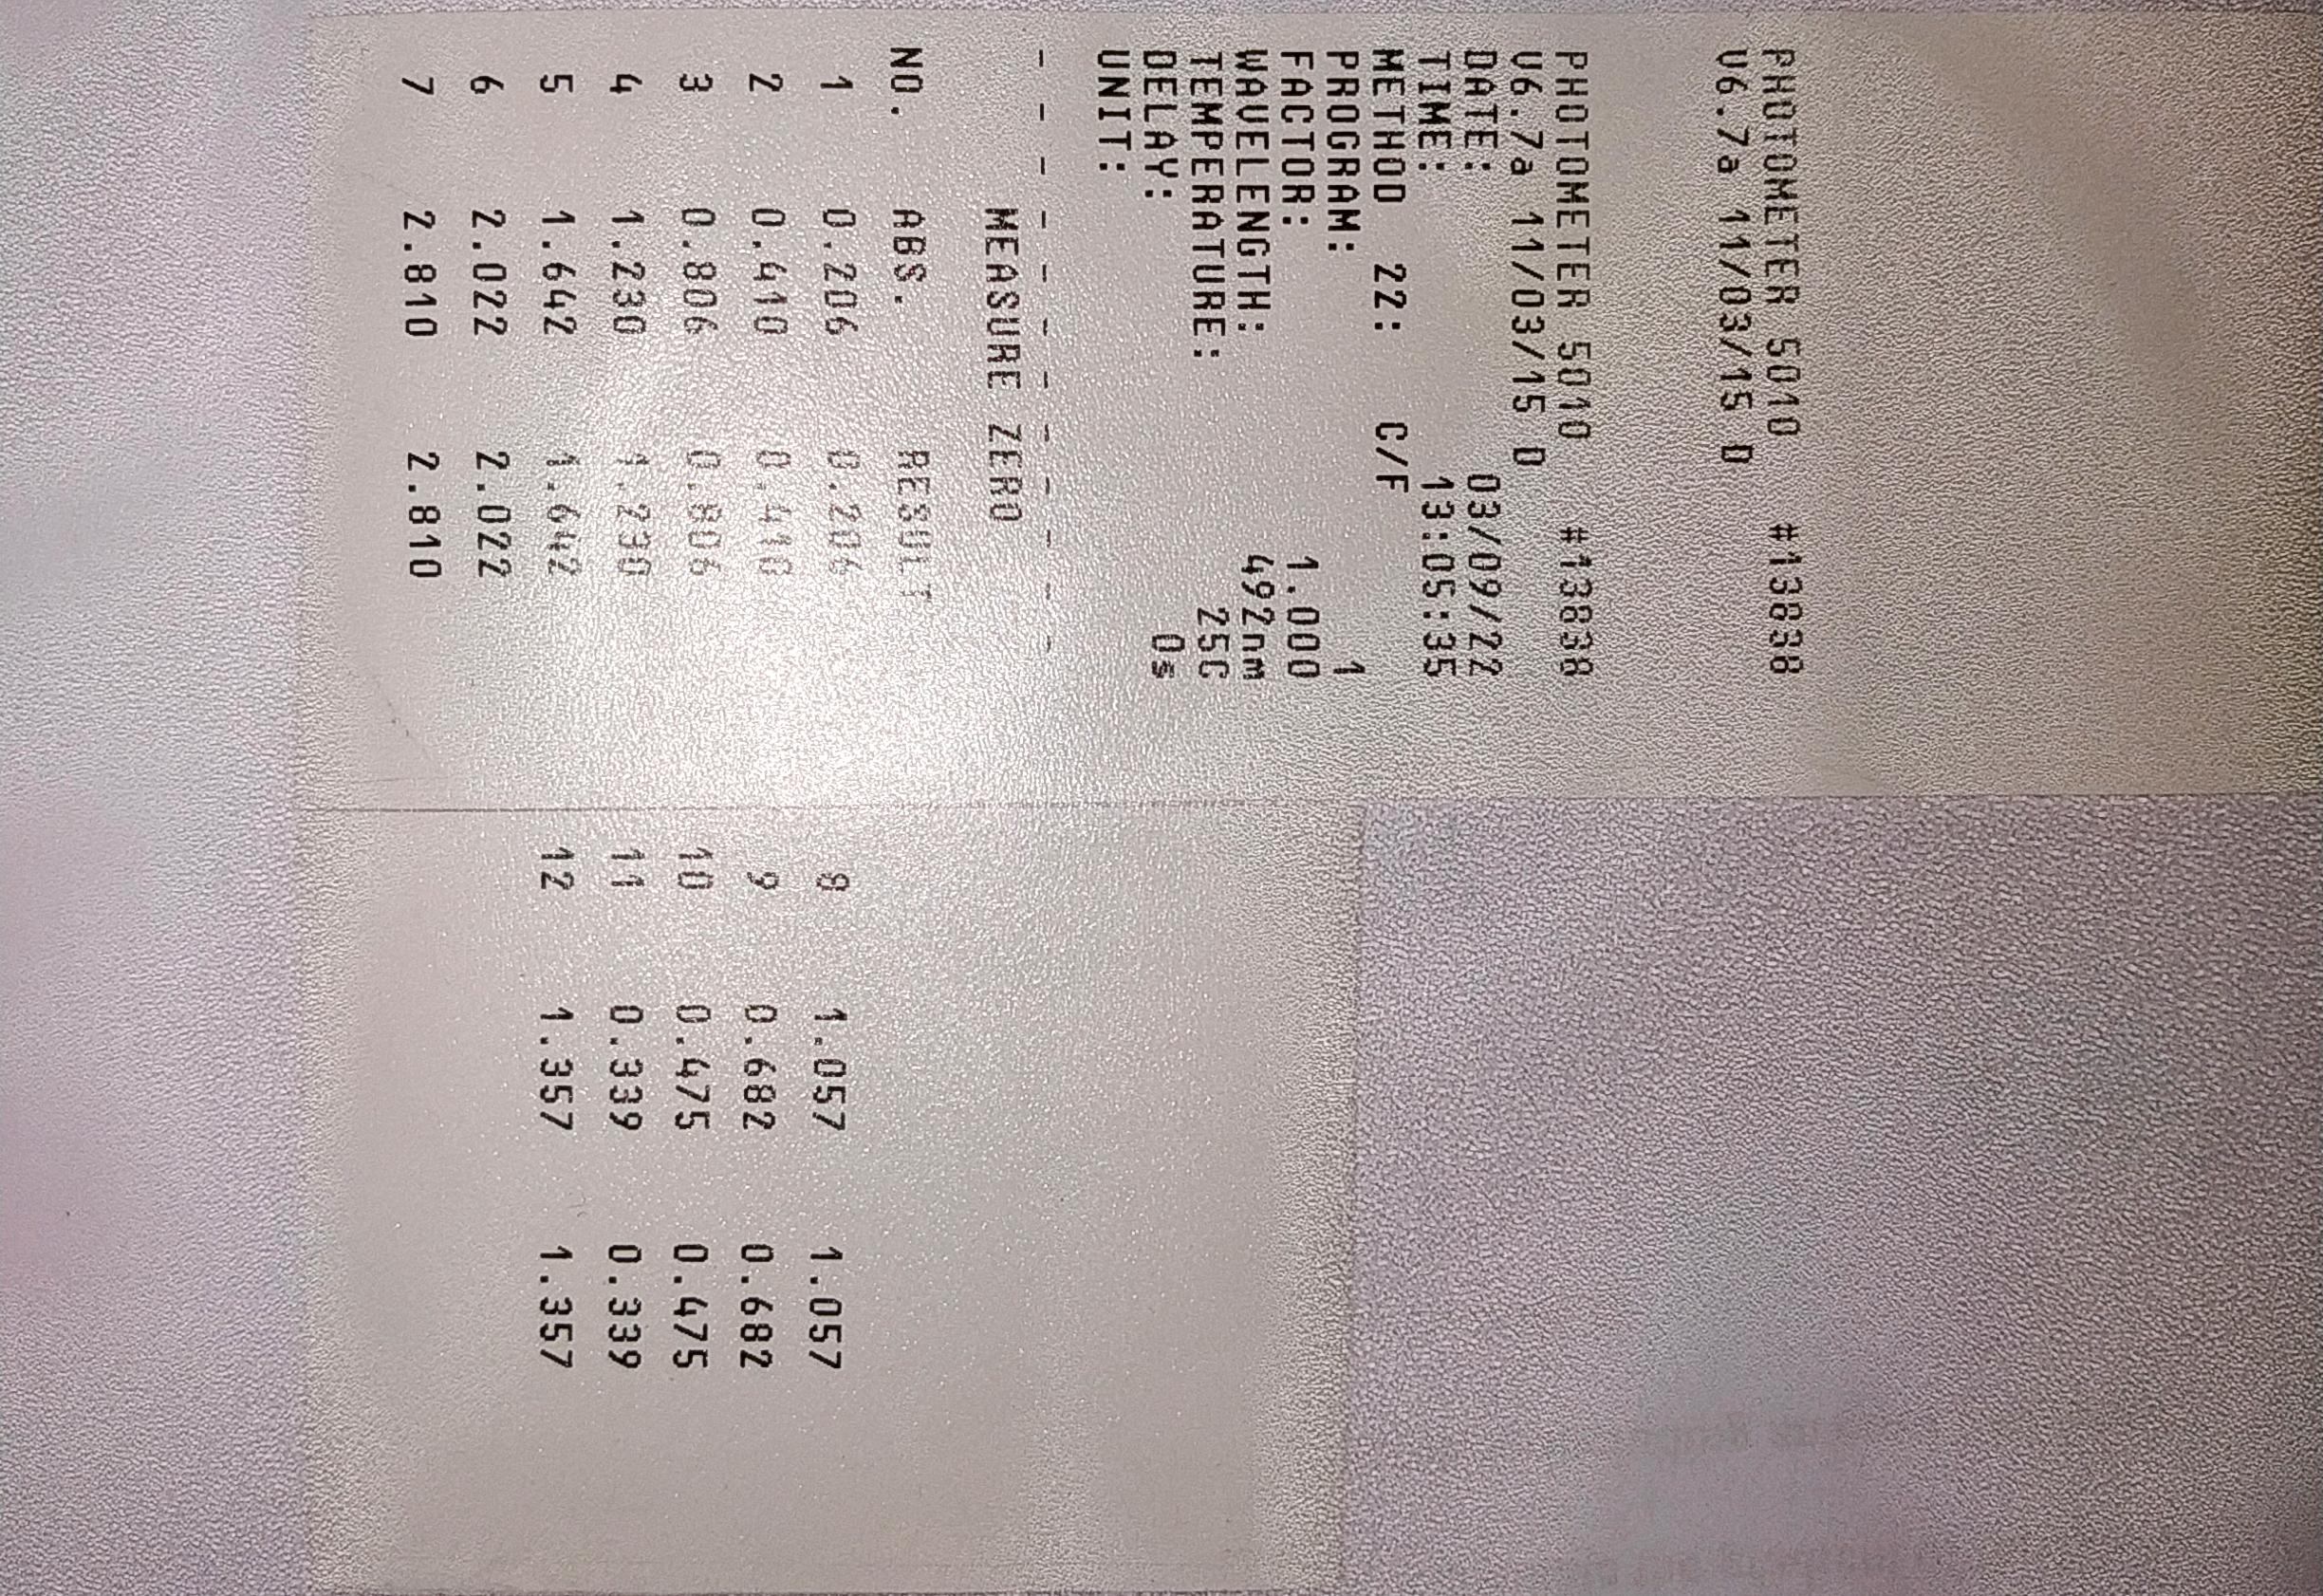
\includegraphics[width=14cm]{2022_03_13 20_01 Office Lens.jpg}
    \caption{Photometer printouts}
    \label{fig:my_label}
\end{figure}
\FloatBarrier
\section{Bibliography}
\begin{thebibliography}{9}
    \bibitem{marker1} \href{https://en.wikipedia.org/wiki/Ammonium_iron(II)_sulfate}{Wikipedia}, consulted 13/03/22
    \bibitem{marker2} \href{https://en.wikipedia.org/wiki/Sodium_acetate}{Wikipedia}, consulted 13/03/22
    \bibitem{marker3} \href{https://en.wikipedia.org/wiki/Hydroxylamine}{Wikipedia}, consulted 13/03/22
    \bibitem{marker4} \href{https://en.wikipedia.org/wiki/Phenanthroline}{Wikipedia}, consulted 13/03/22
    \bibitem{beerlambert} \href{https://en.wikipedia.org/wiki/Absorbance}{Wikipedia}, consulted 13/03/22
\end{thebibliography}


\end{document}
